\subsection{Finding the pupil with Thresholds}
%TEXT
To find the pupil, we have expanded on the \emph{GetPupil(...)} function.\newline
By default, the GetPupil(...) function gathers all contours in the current image. Our assignment was to filter the contours, hopefully ending up with only the pupil.\newline

The optimal result is to have the function return only one contour; the pupil. We found that morphing the image would give us three premises that define a pupil sufficiently accurate: The amount of points making up the contour, its size, and its extension ratio (the contour's area divided by its bounding box)\newline

Before we applied the morphing, we had a very large number of pupil candidates, as seen in the figure below.\newline

\begin{figure}[h]
	\centering
	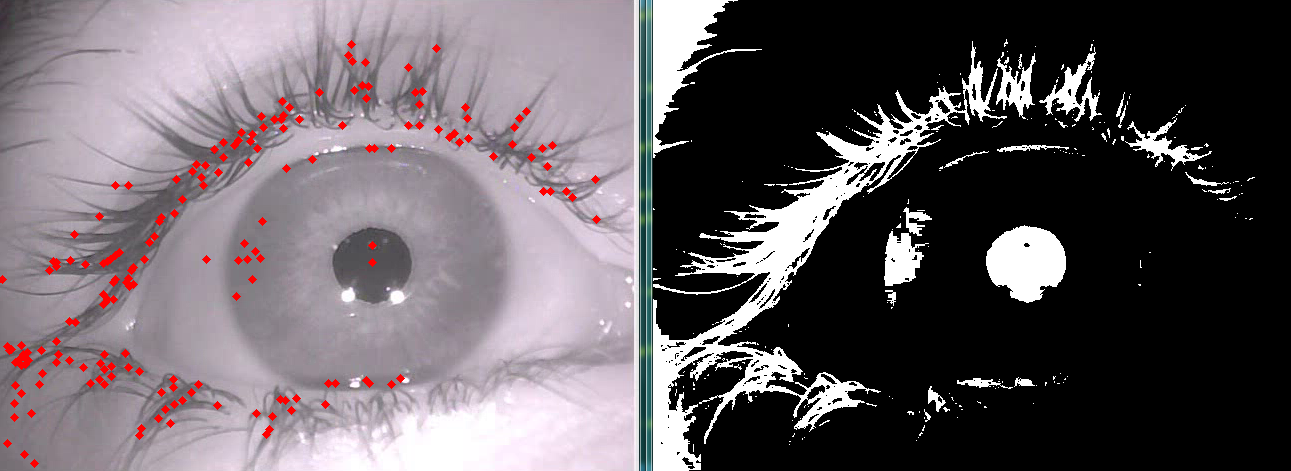
\includegraphics[scale=0.35]{many_pupils.png}
	\caption{The binary image and pupil detection before morphology has been applied.}
\end{figure}

Since any contour is a list of points, connected by lines, we found that one can safely assume that the pupil is a contour made up of at least some amount of points. We found that any contour made up of less than 5 points was certainly not the pupil, hence we setup a filter that disregards all such contours. Since a pupil is circular (or elliptical), a contour made from 5 points would have too few edges, and can therefore be disregarded as a pupil.\newline

Our second filter checks whether the area of the contour is within the minimum and maximum size of the pupil, given by the sliders \emph{minSize} and \emph{maxSize}\footnote{minSize and maxSize are passed as arguments to the GetPupil(...) function.}. These values determine whether a specific contour has an area that is either too large, or too small. This filter is especially useful at filtering minor artifacts and noise that appears in crevices or the like.\newline

The third and final filter checks the contour's extension ratio. Assuming that the pupil is circular, we know that its area \(A_p \approx r^2*\pi\), and the area of its bounding box \(A_b = w*h \approx (2r)^2 \quad | \quad w \approx 2r \wedge h \approx 2r\). Knowing this, we can find out what the standard extension of a circle would be:

\[x = \frac{A_p}{A_b} = \frac{r^2*\pi}{(2r)^2} = \frac{r^2*\pi}{4*r^2}\]

Since the ratio \(\frac{z*x}{z*y} = \frac{x}{y}\), given that \(z = r^2\), we can declare the extension ratio to be \(\frac{\pi}{4}\)
\newline

Alongside our filters, we reduce the number of pupil candidates drastically using morphology.\newline

The morphing is done by dilating the binary image 10 pixels, and then eroding the image 10 pixels. This is known as an \emph{open/close operation}. We do this to remove unnecessary detail that can obstruct our efforts to find the pupil. The open/close operation removes any minor noise and reduces fractioning of contours. It's effects can be seen in the figure below.\newline

\begin{figure}[h]
	\centering
	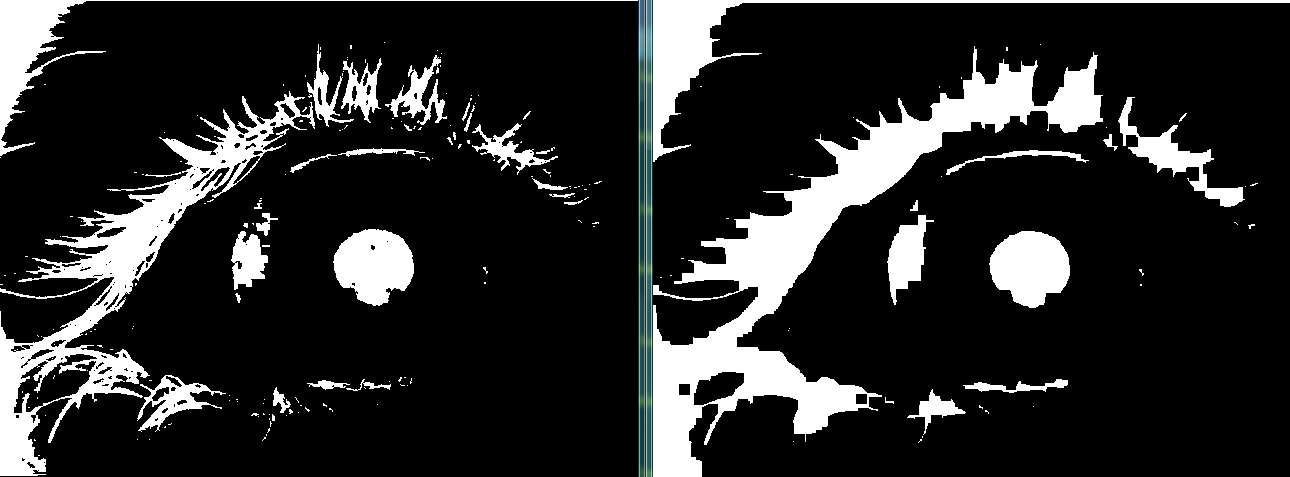
\includegraphics[scale=0.3]{morphology.png}
	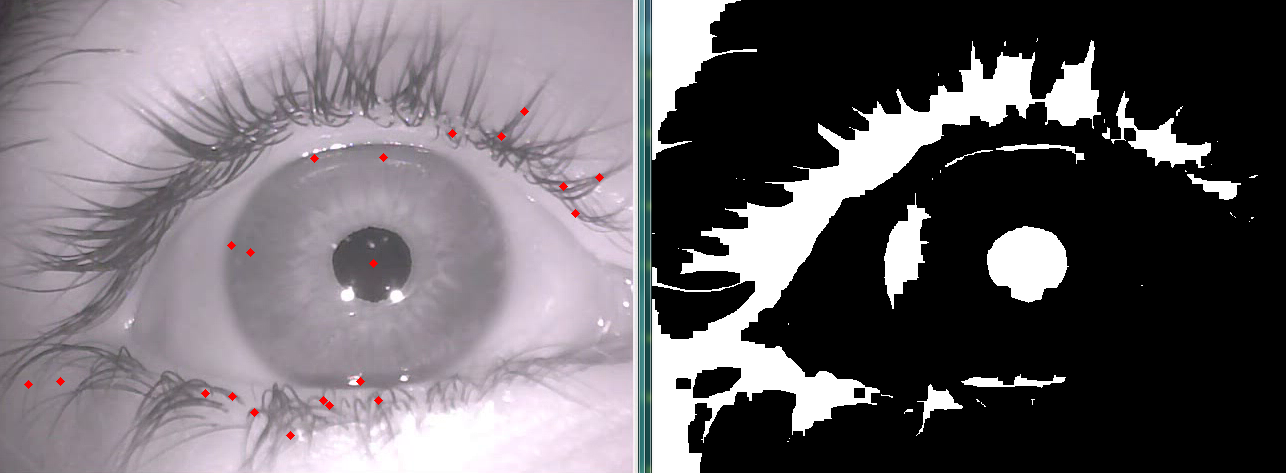
\includegraphics[scale=0.3]{morphology_results.png}
	\caption{The morphology applied to the binary image, and the effect on the pupil tracking.}
\end{figure}

While our efforts does help us reduce the number of potential candidates for the pupil, it is not flawless, and still finds multiple candidates. This is likely due to our premises not being capable of isolating the pupil. Yet, as seen in the figure, the premises and morphology does indeed find the pupil with a fair amount of certainty.
\newline

\subsection{Finding the pupil with Clustering}
The next step after finding the pupil and glints based on thresholds and morphology was to use clustering to segment the image into the regions of interest. For this we used the k-means method based on intensity and position as feature vectors. Playing around with the position or \emph{distanceWeight} we found that changing this value does not give a significant improvement for the segmentation of the pupil. On the other hand, we found that a \emph{k} value of 5 gives a good separation of the pupil as one cluster for the \emph{eye1.avi} sequence, but because of the changes in intensity the same value does not apply for all the sequences.  
(TO-DO 7-10 pupil detection using clustering)
